\documentclass[utf8]{article}
\usepackage{import}
\usepackage{WritingToolsByAcer}

% \excludeversion{WritingMaterials}
% \excludeversion{backup}

\usepackage{chngcntr}
\counterwithout{figure}{section}

%% ================================== acronym ================================= %
\usepackage{acronym}
\newacro{ntic}[NTIC]{non-trivial informational closure}
\newacro{ic}{informational closure}
\newacro{cg}{coarse-grain}
\newacro{cging}{coarse-graining}
\newacro{cged}{coarse-grained}
\newacro{ncg}{neural coarse-graining}
\newacro{OurTheory}[ICT]{Information Closure Theory of Consciousness}


% ============================================================================ %
%                                     Title                                    %
% ============================================================================ %
\title{Information Closure Theory of Consciousness}



% ============================================================================ %
%                                    Authors                                   %
% ============================================================================ %
\author[]{Acer Y.C. Chang\thanks{acercyc@araya.org}}
\author[]{Martin Biehl\thanks{martin@araya.org}}
\author[]{Yen Yu\thanks{yen.yu@araya.org}}
\author[]{Ryota Kanai\thanks{kanair@araya.org }}
\affil[]{ARAYA, Inc., Tokyo, Japan}



% ============================================================================ %
%                                     Body                                     %
% ============================================================================ %
\begin{document}
    \linenumbers
	\maketitle
	\tableofcontents


	\begin{abstract}
		Information processing in neural systems can be described and analysed at multiple spatiotemporal scales. Generally, information at lower levels is more fine-grained and can be coarse-grained in higher levels. However, information processed only at specific levels seems to be available for conscious awareness. We do not have direct experience of information available at the level of individual neurons, which is noisy and highly stochastic. Neither do we have experience of more macro-level interactions such as interpersonal communications. Neurophysiological evidence suggests that conscious experiences co-vary with information encoded in coarse-grained neural states such as the firing pattern of a population of neurons. In this article, we assume that conscious experience is confined due to informational closure from conscious processing to other coarse-grained levels. From this and three additional assumptions, we propose a new computational theory of consciousness: \ac{OurTheory}. \ac{OurTheory} proposes new quantitative definitions of both conscious content and conscious level. With the parsimonious assumptions and simple propositions, \ac{OurTheory} provides explanations and predictions of phenomena associated with consciousness. The implications of \ac{OurTheory} naturally reconciles issues in many existing theories of consciousness and provides explanations for many of our intuitions about consciousness. Most importantly, \ac{OurTheory} indicates that information is the common language bridging consciousness and physical reality. 

		
	\end{abstract}


	\section*{Keywords:}
	Keywords: consciousness, informational closure, neural coarse-graining, level of analysis

            
            
%         \end{ants}    
    
% ============================================================================ %
%                                     Start                                    %
% ============================================================================ %

    \newpage
	\section{Introduction}

		%% Story about a cell
		Imagine you are a neuron in Alice's brain. Your daily work is to collect neurotransmitters through dendrites from other neurons, accumulate membrane potential, and finally send signals to other neurons through action potentials along axons. However, you have no idea that you are one of the neurons in Alice's supplementary motor area and involved in many motor control processes for Alice's action, for example, grabbing a cup. You are ignorant of intentions, goals, and motor plans that Alice has at every moment even though you are part of the physiological substrate responsible for all those actions.
		A similar story also happens to Alice's conscious mind. To grab a cup, for example, Alice is conscious of her intention and visuosensory experience of this action. However, her conscious experience does not reflect the dynamic of your membrane potential or the action potentials you send to other neurons every second. That is, not all information you have is available to Alice's conscious mind.

		%% scale
		
		It seems to be true that we are not consciously accessing information processed at every scale in the neural system. There are both more microscopic and more macroscopic levels than the level corresponding to the conscious contents. On the one hand, dynamics of individual neurons are stochastic \citep{Goldwyn2011, White2000}. However, what we are aware of in our conscious mind shows astonishing stability and robustness against the ubiquitous noise in the neural system \citep{mathis1995computational}. In addition, some parts of the neural system contribute very little to conscious experience (the cerebellum for example \citep{lemon2010life}), also suggesting that conscious contents do not have one-to-one mapping to the entire state of the neural system. On the other hand, human conscious experience is more detailed than just a simple (e.g. binary) process can represent, suggesting that the state space of conscious experience is much larger than what a single overly coarse-grained binary variable can represent. These facts suggest that conscious processes occur at a particular scale. We currently lack a theory to identify the scale which conscious processes correspond to. We refer to this notion as \textbf{the scale problem of consciousness} (Fig.~\ref{fig:scaleproblem}).

		%% our argument
		In this article, we propose a new information-based theory of consciousness, called \ac{OurTheory}. We argue that every process with a high degree of non-trivial information closure (NTIC) has consciousness. This means that the state of such a process corresponds one-to-one to conscious content.\footnote{In the following IC stands for "informational closure" or "informationally closed" and NTIC stands for "non-trivial informational closure" or "non-trivially informationally closed".}. We further postulate that the \textit{level} of consciousness corresponds to the degree of NTIC. (for a discussion of the distinction between level versus content of consciousness see \cite{laureys2005neural, overgaard2010neural}).
		
		In the following, we first introduce non-trivial informational closure and argue for its importance to information processing for human scale agents (Sec.\ref{sec:Non-trivial informational closure}). We next argue that through coarse-graining the neural system can form a high degree of NTIC at a specific coarse-grained level (Sec.\ref{sec:Neural coarse-graining}). In the Sec.\ref{sec:OurTheory}, we propose our theory: \acf{OurTheory}. We also illustrate how \ac{OurTheory} can parsimoniously explain empirical findings from previous consciousness studies (Sec.\ref{sec:Conscious versus Unconscious Processing}) and reconcile several current major theories of consciousness (Sec.\ref{sec:Comparison with other theories}). Finally, we discuss the current theoretical and empirical limitations of \ac{OurTheory} and propose the implications from \ac{OurTheory} to the current consciousness science (Sec.\ref{sec:Limitation and Future work}). 


		\begin{figure}[H]
		    \centering
			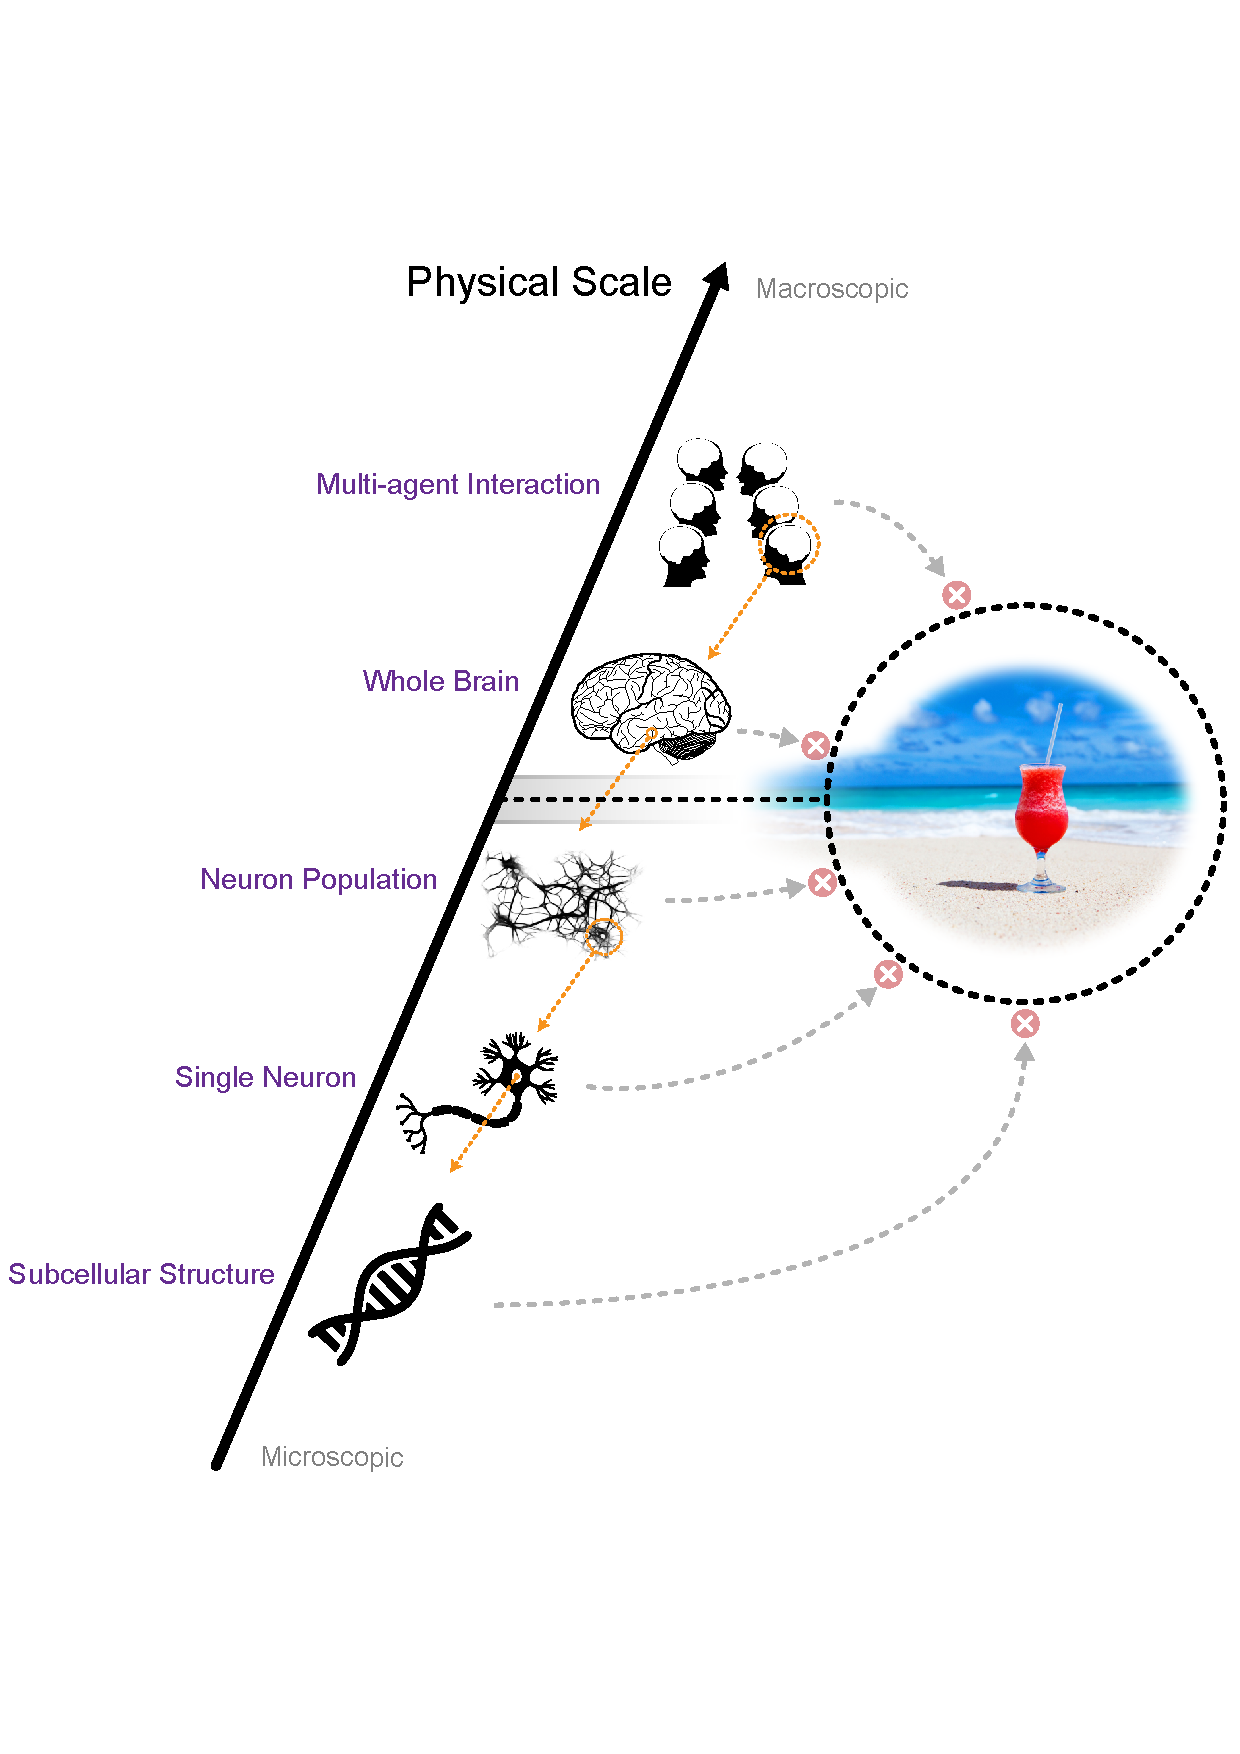
\includegraphics[width=\textwidth]{WritingMaterials/Fig_ScaleProblemOfConsciousness/ScaleProblemOfConsciousness.pdf}
			\caption{The scale problem of consciousness: Human conscious experience does not reflect information from every scale. Only information at a certain coarse-grained scale in the neural system is reflected in consciousness.}
			\label{fig:scaleproblem}
	   	\end{figure}


% ============================================================================ %
%                       Non-trivial informational closure                      %
% ============================================================================ %
	\section{Non-trivial informational closure} \label{sec:Non-trivial informational closure}
		The notion of non-trivial informational closure (NTIC) is introduced by \cite{BERTSCHINGER.2006}. The concept of closure is closely related to system identification in systems theory. One can distinguish a system from its environment by computing the closedness of the system \citep{maturana1991autopoiesis, rosen1991life, pattee2012evolving, luhmann1995probleme}. The closure can be further quantified by information theory.



		% Definition of informational closure
			\noindent
			Consider two processes, the environment process $(E_t)_{t \in \mathbb{N}}$ and the system's process $(Y_t)_{t \in \mathbb{N}}$ and let their interaction be described by the Bayesian network in Fig.~\ref{fig:SystemAndEnv}. Then, information flow $J_{t}$ from the environment $E$ to a system $S$ at time $t$ can be defined as the conditional mutual information $I$ between the current environment state $E_{t}$  and the future system state $Y_{t+1}$ given the current system state $Y_{t}$

				\begin{equation}
    				\label{eq:InformationFlow}
    				\left.\begin{array}
    				{rl}{J_{t}(E \rightarrow Y )} & {:= I(Y_{t+1};E_{t}|Y_{t})} \\
    				%{ } & { \ = H(Y_{t+1}|Y_{t})-H(Y_{t+1}|Y_{t},E_{t})} \\
    				%{ } & { \ = H(E_{t}|Y_{t})-H(Y_{t}|Y_{t},Y_{t+1})} \\
    				%{ } & { \ = H(E_{t}|Y_{t})-H(E_{t}|Y_{t},Y_{t+1})}\\
    				{ } & { \ = I(Y_{t+1};E_{t}) - (I(Y_{t+1};Y_{t})-I(Y_{t+1};Y_{t}|E_{t}))}
    				\end{array}\right.
				\end{equation}

            
				\begin{figure}
					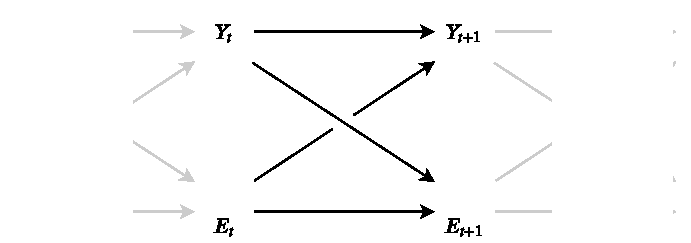
\includegraphics[width=\textwidth]{WritingMaterials/Fig_SystemAndEnv/SystemAndEnv_2.pdf}
					\caption{The dependencies between a system and its environment.} % Figure adapted from \cite{BERTSCHINGER.2006}
					\label{fig:SystemAndEnv}
				\end{figure}


			\noindent
			\cite{BERTSCHINGER.2006} defines that a system is informationally closed when information flow from the environment to the system is zero.

				\begin{equation}
				J_{t}(E \rightarrow Y )=0
				\label{eq:informationflow2}
				\end{equation}


			% ------------------------------- trivial case ------------------------------- %
			\noindent
			Information closure (minimising $J_t$) is trivial if the environment and the system are entirely independent of each other.

				\begin{equation}
				\begin{aligned}
				{I(Y_{t+1};E_{t})=0}&&{\Rightarrow}&&{J_{t}(E \rightarrow Y )=0}
				\end{aligned}
				\end{equation}


			% -------------------------------- non-trivial ------------------------------- %
			\noindent
			However, informational closure can be formed non-trivially. In the non-trivial case, even though a system contains (or encodes) information about the environmental dynamics, the system can still be informationally closed. In such cases, the mutual information between the current states of the environment and the future state of the system is larger than zero. %\footnote{Here we assume that that the environment contains more information than the system, i.e. $H(E|S)>0$ and $E\neq S$}. 

				\begin{equation}
				I(Y_{t+1};E_{t}) > 0
				\end{equation}

			\noindent
			This also implies
				\begin{equation}
					I(Y_{t+1};Y_{t})-I(Y_{t+1};Y_{t}|E_{t}) > 0
				\end{equation}



			\noindent
			And, non-trivial informational closure can be defined as
				\begin{equation}
				\label{eq:NTIC}
    				\left.\begin{array}
    				{rl}{NTIC} & {:=I(Y_{t+1};Y_{t})-I(Y_{t+1};Y_{t}|E_{t})}
    				\end{array} \right.
				\end{equation}
				
				
			\noindent
            The definition can also be re-arranged as 
				\begin{equation}
				\label{eq:NTIC2}
    				\left.\begin{array}
    				{rl}{\qquad} & {\ =I(Y_{t+1};E_{t})-I(Y_{t+1};E_{t}|Y_{t})}
    				\end{array} \right.
				\end{equation}				

			\noindent
			Hence, maximising NTIC amounts to
				\begin{equation}
    				\label{eq:nticObjective}
    				\begin{aligned}
    				& \text{maximising} & { } & I(Y_{t+1};Y_{t}) & { } & \text{and} \\
    				& \text{minimising} & { } & I(Y_{t+1};Y_{t}|E_{t}) & { }
    				\end{aligned}
				\end{equation}
				
			One can also maximise NTIC by 
				\begin{equation}
    				\label{eq:nticObjective2}
    				\begin{aligned}
    				& \text{maximising} & { } & I(Y_{t+1};E_{t}) & { } & \text{and} \\
    				& \text{minimising} & { } & I(Y_{t+1};E_{t}|Y_{t}) & { }
    				\end{aligned}
				\end{equation}			

			\noindent
			This implies the system contains in itself all the information about its own future and the self-predictive information contains the information about the environment. Therefore, to form NTIC, the system can internalise and synchronise with the dynamics of the environment, i.e. model the environment. Furthermore, having high degrees of NTIC entails having high predictive power about the environment. This gives biological agents a great functional and evolutionary advantage. 
			

% ============================================================================ %
%                            Neural coarse-graining                            %
% ============================================================================ %
	\section{Coarse-graining in the Neural System} \label{sec:Neural coarse-graining}

		%% stochasticity at microscopic levels
		The formation of NTIC with a  highly stochastic process is challenging. NTIC requires the predictability of the system state and is therefore impeded by noise in the system. Information processing at the microscopic levels (the cellular levels) in neural systems suffer from multiple environmental noise sources such as sensor, cellular, electrical, and synaptic noises. For example, neurons exhibit large trial-to-trial variability at the cellular level, and are subject to thermal fluctuations and other physical noises \citep{faisal2008noise}. 
		
  
        %% Our argument
		However, it is possible that neural systems form NTIC at certain macroscopic levels through coarse-graining of microscopic neural states.
		
		Coarse-graining refers to many-to-one functions which aggregate microscopic states to a macroscopic state. In other words, a number of different micro-states correspond to the same value of the macro-variable \citep{price2007causation}. Coarse-grainings, can therefore form more stable and deterministic state transitions and more often form NTIC processes. 
		
		For neural systems this means that a microscopically noisy neural system may still give rise to an NTIC process
		on a more macroscopic scale.
		
		In neural systems such coarse-grainings have been observed to represent external stimuli in empirical studies.
		

		=== so, to here, it's fine ===
		Because coarse-graining is an effective way to create stable variables, a stochastic system (e.g., neural systems) can represent information stably by encoding information using coarse-grained macroscopic variables. 
		
		============================================================================
		
		Indeed, empirical evidence suggests that coarse-graining is a common coding strategy to establish robustness against noise at microscopic levels of the neural system. For instance, the inter-spike intervals of an individual neuron are stochastic. This implies that the state of an individual neuron does not represent stable information. However, the firing rate, i.e. the average spike counts over a given time interval, is more stable and robust against noise such as the variability in inter-spike intervals. Using this temporal coarse-graining strategy, known as rate coding \citep{adrian1926impulses, gerstner2002spiking, maass2001pulsed, panzeri2015neural, stein2005neuronal}, neurons can encode stimulus intensity by increasing or decreasing the firing rate \citep{kandel2000principles}. \citep{stein2005neuronal}. The robustness of the rate coding is a direct consequence of the many to one mapping (i.e., coarse-graining).
		
		% population code
		Population coding is another example of encoding information through coarse-graining in neural systems. In this coding scheme, information is encoded by activation patterns of a set of neurons (a neuron population). In the population coding scheme, many states for a neuron population map to the same state of encoded information, thereby reducing the influence of noise in individual neurons. That is, stable representations can be formed through coarse-graining the high dimensional state space of a neuron population to a lower dimensional macroscopic state space \citep{kristan1997population, pouget2000information, binder2009encyclopedia, QuianQuiroga2009}. Therefore, individual neuron states (the microscopic level) are not informative enough about the full encoded contents at the population level (the macroscopic level). Instead, coarse-grained variables are better substrates for stably encoding information and allow the neural system to ignore noisy interactions at the fine-grained level \citep{Woodward2007-WOOCWA}.
		
        These two examples show that the known coding schemes can be viewed as coarse-graining, and provide stochastic neural systems with the ability to form more stable and deterministic macroscopic processes for encoding and processing information reliably. We argue that through coarse-graining the neural systems is able to form NTIC processes at macroscopic levels. Based on the merit of coarse-graining in neural systems, We propose a theory of consciousness in the next section. 


			
			
% 		% neural coarse-graining by Nic
% 		The practical implementation mentioned above suggests that  NTIC can be formed by coarse-graining sensory inputs in artificial neural networks. \citep{guttenberg2016neural} proposed a "neural coarse-graining (NCG)" architecture which aims to capture the emergent large-scale dynamics in the environment. The NCG network learns to coarse-grain input signals and extract latent variables which are both predictive and predictable in the input signal and therefore form NTIC.




% ============================================================================ %
%               A neural coarse graining theory of consciousness               %
% ============================================================================ %
	\section{\acf{OurTheory}}\label{sec:OurTheory}
	
        In this section, we propose a new theoretical framework of consciousness: \acf{OurTheory}.  In \ac{OurTheory}, we claim that being NTIC is sufficient for a process to be conscious. The implications of \ac{OurTheory} will be discussed in Sec.~\ref{sec:cl}, \ref{sec:cc}, and \ref{sec:reconcile}. In what follows, we will first establish four assumptions on which \ac{OurTheory} depends, and then develop the specific propositions of \ac{OurTheory} in detail. 
        
        The first assumption is that every human conscious percept is informative. Here, "informative" refers to the resolution of uncertainty. Being in a certain conscious state rules out a number of other possible conscious states. This is in line with the impression that our conscious experience consist of multi-dimensional information and usually involves information from multiple modalities. Therefore, every human conscious percept resolves some amount of uncertainty and provides information.  
        
        This assumption is also in agreement with the "axiom" of \textit{information} in Integrated Information Theory (IIT 3.0) which claims that \myQuote{...an experience of pure darkness is what it is by differing, in its particular way, from an immense number of other possible experiences...} \citep[p.2]{oizumi2014phenomenology}.
        
        Second, we further assume that all information requires physical substrates. 
        From these two assumptions, it follows that the amount of (self-)information possessed by a conscious percept must be equal to the (self-)information of a particular event or entity in the physical reality. 
        
        In this theory, we consider information is the common language between conscious experience and the physical reality. This means that consciousness is fundamentally associated with information \citep{chalmers1996conscious, tononi2004information, gamez2011information, Gamez2016}).
        
        === How about if I change this ===
        The third assumption is that no consciousness can contain complete information about the universe. This means that there exists a informational boundary for every consciousness, i.e. informationally closed to the the universe. This is in line with our conscious experience that information provided by every conscious percept is limited.
        
        === to this ===
        The third assumption is that there exists a informational boundary for every consciousness. The informational boundary here means that no consciousness can contain information of the entire universe and every consciousness is informationally closed to the the universe. This is in line with our conscious experience that information provided by every conscious percept is limited.
    
        Together with the first three assumptions, this means that the physical representations of the contents of any consciousness must be a coarse-graining of the universe states and also informationally closed to the universe.
        
        Note that a coarse-grained process $Y$ can be a coarse-graining of another coarse-grained process $S$ of the universe $X$ (see Fig.~\ref{fig:fullgraph}). Here, we consider $S$ as a coarse-graining of $X$ and call it the system. Then $Y$ is a coarse-graining of the system $S$. We can then also define another coarse-graining of $X$ called the environment $E$ of $S$. This is the coarse-graining that contains the information about $X$ that is not contained in $S$. Importantly, in this case, if a macroscopic process $Y$ is informationally closed to the universe $X$, this implies $Y$ is also informationally closed to both the system $S$ and the environment $E$. 
        
            \needhelp{@Martin, if you think it's better to have a proof for this and if you don't mind, you can help me to write the proof here or create an appendix section and put it there. If you have no time, I can also do this.}
		\begin{equation}
			\label{eq:ICchain}
			\begin{aligned}
		    & I(Y_{t+1};X_t|Y_{t})=0 & \implies & I(Y_{t+1};S_t|Y_{t})=0 \\
		    & {} & \implies & I(Y_{t+1};E_t|Y_{t})=0
			\end{aligned}
		\end{equation}
		
        
        This results in a crucial implication that informational closure can occur between levels in a system. The macroscopic level $Y$ can be informationally closed to its microscopic level $S$ within a system \citep{PFANTE.2014}.

		\begin{figure}[H]
		    \centering
			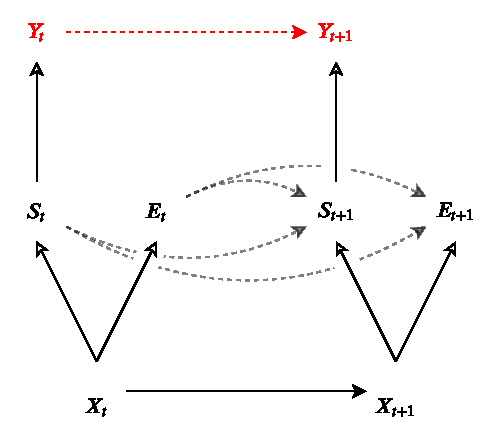
\includegraphics[width=\textwidth]{WritingMaterials/Fig_FullGraph/FullGraph.pdf}
			\caption{The information flow amounts the universe $X$, the system $S$, the environment of the system $E$, and the coarse-grained process of the system $S$. The solid line with a filled arrow from $X_t$ to $X_{t+1}$ represents the microscopic dynamic of the universe. The solid lines with a empty arrow represent directions of coarse-graining. The dashed lines represents virtual dependencies between  two macroscopic variables. The red $Y_t$, $Y_{t+1}$, and the red dashed line in between represents a macroscopic process which forms informational closure at a certain coarse-grained level.}
			\label{fig:fullgraph}
	   	\end{figure}
       
        A concrete example in the context of neuroscience is that $X$ represents the microscopic level of the universe, $S$ a cellular level process in the neural system, $Y$ a more macroscopic process of the neural system coarse-grained from the cellular level process $S$, and $E$ the environment which the cellular level process $S$ interacts with. The environment $E$ may includes other processes in the neural system, the sensors for perception and interoception, and external physical worlds, respectively.	   	
        
        Our fourth assumption is that information provided by every conscious content is not trivial. More precisely, there exists a certain degree of mutual information between conscious processes and the environments which it interacts with. As mentioned in Sec.\ref{sec:Non-trivial informational closure} a process can be informationally closed to another one and still have mutual information with it, i.e. be NTIC. Therefore, a macroscopic process $Y$ can be NTIC to the system's environment $E$ and at the same time be informationally closed to its microscopic process $S$. In other words, the macroscopic process can encode environmental information (by forming NTIC) and, however, be ignorant to its microscopic processes (IC). This is in line with our conscious experience that information that every conscious percept provides represent rich and structured environmental states without involving much information at microscopic activities.
        
        Finally, together with the four assumptions above, our main proposition is that the coarse-graining that physically represent consciousnesses are those that are informationally closed with respect to the universe states and concurrently be NTIC with respect to its environment. More formally this means that every NTIC process $Y_t$ at time $t$ corresponds to a conscious process $C_t=\{C_t^{Content},C_t^{Level}\}$ such that the content $C_{t}^{Content}$ of $C_t$ is just $Y_t$:
		\begin{equation}\label{eq:cContent}
			C_{t}^{Content} = Y_{t}.
		\end{equation}
		
		
		\noindent
        We further propose that the level of consciousness $C_{t}^{Level}$ can be measured by the degree of $NTIC_{t}$ of $Y_t$:
		\begin{equation}\label{eq:cLevel}
			C_{t}^{Level} = NTIC_{t}.
		\end{equation}
		We discuss the implications of these propositions in the following. 	
		
		
		% ---------------------------------------------------------------------------- %
        %        Level of Consciousness correlates degrees of NTIC of a process        %
        % ---------------------------------------------------------------------------- %
	    \subsection{Level of Consciousness is equal to the degree of NTIC of a process}\label{sec:cl}
            
            According to Eq.~\ref{eq:nticObjective}, \ac{OurTheory} implies that conscious levels are determined by two quantities. 
            
            First, to form a high level of NTIC, one can increase the mutual information $I(Y_{t+1};Y_{t})$ between the current internal state $Y_t$ and the future internal state $Y_{t+1}$. In other words, conscious levels are associated with the degree of self-predictive information. This mutual information term can be further decomposed to two information entropy quantities: 
            
            \begin{equation}
            \label{eq:SelfEntropy}
            I(Y_{t+1};Y_{t}) = H(Y_{t+1}) - H(Y_{t+1}|Y_t)
            \end{equation}
            
            This implies that a highly NTIC process must have rich dynamics with self-predictability over time. Another implication is that complex systems can potentially attain a higher level of consciousness due to the larger information capacity needed to attain high mutual information. This outcome is consistent with the common intuition that conscious levels are associated with the degree of complexity of the system.
    
    	    Second, one can minimise the conditional mutual information $I(Y_{t+1};Y_{t}|E_{t})$ to increase the level of NTIC. This quantity suggests that conscious level increases with the amount of information about the environment state $E_t$ that the NTIC process encodes in its own state $Y_t$. An important implication is that agents interacting with a complex environment have the chance to build a higher level of NTIC within their systems than those living in a simple environment. In other words, the level of consciousness is constrained by environmental complexity. 
    	   
    	    %% not monotonic
    		It is important to note that NTIC can be a non-monotonic function of the scale of coarse-graining. We saw above that not sufficiently coarse-grained variables have low values of NTIC. On the other hand, overly coarse-grained macroscopic variables  also result in low values of NTIC. For example, in an extreme scenario, when all microscopic states map to a single macroscopic variable, the macroscopic level does not have any information capacity and thus cannot have high mutual information across time steps.  Therefor, only processes at a certain level of coarse-graining in the neural system can form a high degree of NTIC (Fig.~\ref{fig:LevelOfConsciousness}). \ac{OurTheory} indicates that consciousness occurs at the intermediate level of coarse-graining where the maximal NTIC is formed within the neural system. 
    		
    		\begin{figure}[H]				
        		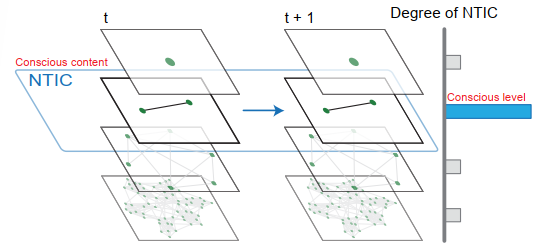
\includegraphics[width=\textwidth]{WritingMaterials/Fig_temp/FoxitReader_2019-01-31_19-03-59.png}
        		\caption{A n1on-monotonic relationship between Level of coarse-graining and level of consciousness.}
        		\label{fig:LevelOfConsciousness}
    		\end{figure}
            
            
            % Finally, which coarse-grained level can form high NTIC? 
            % agent-scale operation
            % At the physical scale which human being interact with, the environmental dynamics is nearly deterministic following the laws of classical physics. It gives agents interact at this physical scale great advantages if the agents can build NTIC process internally. Therefore, to coarse-grain microscopic states is necessary
    	   
            % %% Link to consciousness
            % At the physical scale which human beings live in, the environmental dynamics is nearly deterministic following the laws of classical physics. This suggests that information in the environment is nearly closed at the right spatio-temporal scale. Therefore, this gives agents living at this physical scale great advantages if the agents form an NTIC process internally. Therefore, coarse-graining becomes necessary to map microscopic sensory and neuronal states into macroscopic NTIC process. 
            	   
    			
		\subsection{Conscious Contents Corresponding to States of a NTIC process}\label{sec:cc}
    	    % richness 
    		\ac{OurTheory} proposes that conscious contents correspond to the states of NTIC processes (Eq.~\ref{eq:cContent}). This implies that the size of the state space of an NTIC process is associated with the richness of conscious contents that the process can potentially have. Therefore, a complex NTIC process with a high dimensional state space can have richer conscious experience than a simple NTIC process can have. This outcome is consistent with the intuition that the richness of conscious contents is associated with the complexity of a system. 
    		
    		% CC doesn't include all microscopic states
    		As mentioned above, informational closure can happen between scales of coarse-graining within a single system. Thus, a macroscopic NTIC process can be ignorant to its microscopic states. \ac{OurTheory} argues that human conscious contents do not reflect cellular level activity because the conscious process which corresponds to a macroscopic NTIC process is informationally closed to the cellular level in the human neural system. Further more, since NTIC processes are informationally closed, each of them can be considered as a reality. In the extreme case, when the information flow from the its microscopic processes and environment is completely zero (Eq.~\ref{eq:informationflow2}), the future states of the process is only determined by its past states. 
    		
    		Importantly, NTIC processes encodes environmental information in its state. This suggests that a NTIC process can be considered as a process that simulates the environmental dynamics. This implication fit well with some other theories of consciousness (for example, world simulation metaphor ~\citep{revonsuo2006inner}). Note that \ac{OurTheory} doesn't assume that generative models are necessary for consciousness. The implication a natural consequence based on our proposition. 
            
            Finally, a coarse-graining is a many to one map from microscopic to macroscopic states and \ac{OurTheory} proposes that conscious contents $C_{t}^{Content}$ is the state of the NTIC process $Y_t$. Therefore, \ac{OurTheory} implies multiple realisation thesis of consciousness \citep{putnam1967psychological,bechtel1999multiple} which suggests that different physical implementations could map to the same conscious experience.
            
            
		% ---------------------------------------------------------------------------- %
        %             Reconciling the levels and contents of consciousness             %
        % ---------------------------------------------------------------------------- %
	    \subsection{Reconciling the levels and contents of consciousness}\label{sec:reconcile}
    	    While it is useful to distinguish the notion of the  levels and contents of consciousness, whether they can be clearly dissociated has been a matter of debate \citep{bayne2016there, Fazekas2016}. In \ac{OurTheory}, conscious levels and conscious contents are just two different properties of NTIC processes, and, therefore, naturally reconciles the two aspects of consciousness. In an NTIC process with a large state space, conscious contents consist of rich and high dimensional information. Therefore, this framework integrates the levels and the contents of consciousness in a coherent fashion by providing explicit formal definitions of the two notions.  
    	    
    	    
    	    According to Sec.~\ref{sec:cl} and Sec.~\ref{sec:cc}, an important implication from \ac{OurTheory} is that both conscious levels and conscious contents are associated with the entropy $H(Y)$ of an NTIC process, and therefore the size of the state space. To form a high degree of NTIC for rich conscious contents, the process needs to have a large state space and also the capacity of predictive information   (Eq.~\ref{eq:nticObjective}).
    	    \ac{OurTheory} therefore explains why in normal physiological states conscious levels and conscious contents are positively correlated \citep{laureys2005neural}. This implication is also in line with the intuition in which consciousness is often associated with complex systems.
    			
            % ---------------------------------------------------------------------------- %
            %                              Dynamical Boundary                              %
            % ---------------------------------------------------------------------------- %
            % \subsection{Dynamical Boundary}
            % Our theory predicts that the boundary of a conscious system is dynamical. The boundary is determined by the NTIC process. This implies that when the structure of interaction between variables changes the physical boundaries supporting consciousness should also change. If some coarse-grained variables encode environmental information, they may become necessary components to form high NTIC. In such case, these coarse-grained variables are "recruited" inside the boundary of conscious processes. Note that, due to synergistic information, even recruiting some new variables may largely increase the level of NTIC. 
            % This may explain why consciousness is tightly associated with binding and integration of information in human perception and cognition. Another crucial implication is that the same neural substrates may not be always involved in conscious processing rather it depends on whether it creates high NTIC with other members in the neural system. \needfig{Maybe I need a figure here as well}
    
    
    % ============================================================================ %
    %                    Conscious versus Unconscious Processing                   %
    % ============================================================================ %
	\section{Conscious versus Unconscious Processing}\label{sec:Conscious versus Unconscious Processing}
	    In this section, we show how \ac{OurTheory} can make predictions about what processes are conscious and what are unconscious. \ac{OurTheory} is constructed using information theory. Therefore, \ac{OurTheory} can provide predictions based on the mathematical definitions. In the end of this section, we discuss a critical implication of \ac{OurTheory} for neuroscience research on consciousness.  
	    
        % While our theory is built upon a minimal set of assumptions, it possesses predictive power about the relationship between information processing in the neural system and conscious experience.
	    
        % 		Our theory argues that, to make information conscious, the following necessary and sufficient conditions need to be satisfied.
        
        %         We especially highlight the second condition because it is critically related to many empirical research results even though it is only a necessary condition. As we will describe below, this theory can well explain a variety of previous empirical findings in consciousness science and further make predictions for future research. In this section, we discuss how the two informational-based conditions link to conscious experience. 
		
		
		
        % ---------------------------------------------------------------------------- %
        %                            Unconscious Processing                            %
        % ---------------------------------------------------------------------------- %
        \subsection{Unconscious Processing}
            In this section, we highlight two scenarios in which the degree of NTIC is rendered low for a process, and thereby making the process unconscious.
        
            \subsubsection*{Informational is not Closed}\label{sec:reflexive}
                If a process is not informationally closed, the degree of NTIC is low (Eq.~\ref{eq:nticObjective2}) resulting in low or no consciousness. In such cases, the current state of a process depends primarily on the environment state (see Fig.~\ref{fig:reflexive}), but receives little influence from its past state. Reflexive behaviours \citep{casali2013theoretically} can be considered an example of this scenario. In \ac{OurTheory}, if we can view reflexive behaviours as situations in which the internal state $Y_t$, which triggers reflexive action, is determined by the environment state $E_{t-1}$ overruling the influences from its own past $Y_{t-1}$.  Such interpretation of reflexive behaviour from the viewpoint of \ac{OurTheory} naturally explains why reflexes do not involve conscious experience of external stimuli. 

             	% reflexive behaviour
        		\begin{figure}[H]
        			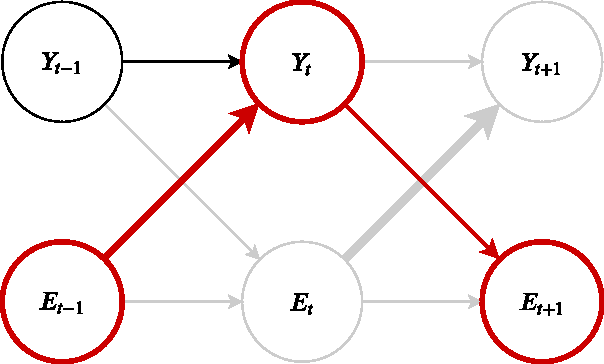
\includegraphics[width=0.8\textwidth]{WritingMaterials/Fig_Reflexive/Reflexive.pdf}
        			\caption{
        			    A diagram depicting the information flow in reflexive behaviours (shown by the red nodes and arrows) happening through the interaction between a process $Y$ and its environment $E$. In such situations, the internal state $Y_t$ is mostly dependent on the environment state $E_{t-1}$ but less on its past state $Y_{t-1}$. Therefore, the process $Y$ is not informational closed. As a  consequence, $Y$ is unable to form high NTIC and, therefore, remain unconscious. 
        			    }
        			\label{fig:reflexive}
        		\end{figure}  
        		
        		The same principle can be applied to interpret blindsight \citep{humphrey1999history, humphrey1974vision, Humphrey1970} and procedural memory \citep{doyon2009contributions, ashby2010cortical} which are often considered as unconscious processes. Blindsight patients are able to track objects, avoid obstacles, and make above chance-level visual judgements without having any conscious perception about visual stimuli. We argue that action outputs of blindsight can be directly guided by sensory inputs through stimulus-response maps. The neural circuits are not informationally closed and, therefore, unconscious. Similarly, for procedural memory, the state transitions of action controls largely depends on the concurrent environmental states. This prevents the internal processes of procedure memory from informational closure and being conscious. \ac{OurTheory} also offer an interpretation as to why patients with visual apperceptive agnosia \citep{james2003ventral} can perform online motor controls without visual awareness of action targets \citep{10.3389/fneur.2014.00255}. 

        		
        		\ideaCallout{Mayeb can put in theory part}
        		As we have seen in the examples above, a crucial implication of \ac{OurTheory} is that a pure feedforward network cannot produce consciousness because NTIC requires a form of memory $I(Y_{t+1};Y_{t})$. Without memory, a network's current state is entirely driven by the input the network receives from the environment without any influence from its own past states. Therefore, such a network is incapable of forming an NTIC. In contrast, a network with recurrent loops can maintain information about its own past states. This forms an information channel between the past and the future states of the network and, thus, makes the network capable of being informationally closed. This result coincides with theories of consciousness emphasising the importance of recurrent circuits to consciousness \citep{lamme2006towards, edelman1992bright, tononi2008neural}.
        		
                % However, we derive this conclusion from a more fundamental informational-related hypothesis indicating the more generalised principle behind it. 


            \subsubsection*{Information is Trivial}
                According to \ac{OurTheory}, when encoded information in a process is trivial, i.e. no mutual information between the process states and its environment states $I(Y_{t+1};E_{t})$ (Eq.~\ref{eq:nticObjective2}), this could lead low NTIC. In such case, this process is considered to be unconscious due to the low level of NTIC. This implies an isolated process which is simply informationally closed is insufficient to be conscious. 
                This mathematical property of \ac{OurTheory} provides a natural and intuitive (but only partial, see the current challenge in  Sec.~\ref{sec:Limitation and Future work}) solution to the boundary and the individuality problem of consciousness
                    \footnote{The boundary problem of consciousness refers to identifying physical boundaries of conscious processes and the individuality problem of consciousness refers to identifying individual consciousnesses in the universe.}
                \citep{Raymont2006-RAYUOC}. Consider a NTIC process $Y$ and an isolated informationally closed process $\hat{Y}$ with only trivial information. Adding $\hat{Y}$ to $Y$ can still keep informational closure, but, however, does not increase non-trivial information, i.e. doesn't affect consciousness. 
                
    			\begin{equation}
    			    \begin{aligned}
                        I(Y,\hat{Y};E) & = H(Y,\hat{Y}) - H(Y,\hat{Y}|E) \\
                                       & = H(Y) + H(\hat{Y}|Y) - (H(Y|E)+H(\hat{Y}|Y,E)) \\
                                       & = H(Y) + H(\hat{Y}) - (H(Y|E)+H(\hat{Y})) \\
                                       & = H(Y) - H(Y|E)\\
                                       & = I(Y;E)				
    				\end{aligned}
    			\end{equation}
                
                This implies that isolated processes with trivial information do not contribute consciousness and should be considered being outside the information boundary of the conscious processing (for more details of the boundary detection procedure, see \cite{krakauer2014information}). 
                This property also implies that consciousnesses do not emerge from just aggregating informationally closed (isolated) processes which contain trivial information.\footnote{However, we do not exclude the possibility that triviality of encoded information is just a proxy of other quantities which more directly associate with consciousness. We point out that this is a limitation of the current version of \ac{OurTheory} in Sec.~\ref{sec:Limitation and Future work}.}
                
                
                



        % ---------------------------------------------------------------------------- %
        %                             Conscious Processing                             %
        % ---------------------------------------------------------------------------- %
		\subsection{Conscious Processing}\label{sec:conscious processing}
		    According to \ac{OurTheory}, NTIC is sufficient for a process to be conscious. We claim that any process, system, or cognitive function which involves any NTIC process should be accompanied by conscious experience. 
		    
		    Previous consciousness research has identified a number of diverse cognitive processes often accompanied by conscious experience. \ac{OurTheory} provides an integrated account for why these processes involve conscious experience. NTIC processes encode environmental information into its own states and dynamics. Therefore, An NTIC process can be seen as an internal simulation engine for the agent-environmental interactions \citep{BERTSCHINGER.2006}. Information from NTIC processes is essential for several cognitive processes. 
		    
		  %  NTIC is a powerful property in the context of evolution. NTIC processes encode environmental information into its own states and dynamics. Hence, an NTIC process can be seen as a simulation engine of the environment \citep{BERTSCHINGER.2006}. Therefore, NTIC processes can provides valuable information for survival as a basis of several cognitive functions. 
		    
		    One of the most valuable information is the predictions about the environmental states. Cognitive functions requiring agent-scale environmental predictions are likely to recruit NTIC processes and therefore accompanied by conscious experience, for example planning and achieving long term goals.
		   
            Second, as a simulation engine, with a given initial state, an NTIC process can self-evolve and simulate the environmental transitions. Cognitive functions involving simulations are expected to involve NTIC processes. Consequently, mental simulation, imagination, computing alternative realities, and generating counterfactuals often come with conscious experience. 
            
    	    Third, as an informationally closed system, an NTIC process can still provide environmental information without new sensory inputs. This is crucial for many types of off-line processing. Therefore, in contrast to reflex-like behaviours mentioned above (Sec.~\ref{sec:reflexive}), behaviours requiring off-line computations \citep{milner1999paradoxical, himmelbach2005dorsal,revol2003pointing} often involve conscious experience. 
    	    
    	    Finally, for agents adapting to complex environments (e.g., human being), any state of the NTIC process can be seen as an integration of high dimensional information. To accurately encode information about the complex environmental states and transitions, the NTIC process requires knowledge about the complex causal dependencies involved in the environment. Therefore, cognitive functions requiring large scale integration are likely to involve NTIC processes and accompanied by conscious experience. % Furthermore, the high dimensional integrated information is also critical for an agent to learn new behaviours to achieve flexibility and the strategic behavioural controls and decision-making. 
    	    
    	    Note that many of the claims above are compatible with several theories of consciousness which highlight the connection between consciousness and internal simulation, predictive mechanism, or generative models inside a system (e.g. world simulation metaphor ~\citep{revonsuo2006inner}, predictive processing and Bayesian brain~\citep{clark_2013,Hohwy2013,SethPP2014}, generative model and information generation~\citep{kanai_chang_yu_de_abril_biehl_guttenberg_2019}). Instead of relating functional or mechanistic aspects of a system to consciousness, \ac{OurTheory} captures common informational properties underlying those cognitive functions associated with consciousness. As such, \ac{OurTheory} does not assume any functionalist perspective of consciousness, which associate specific functions to consciousness.  That is to say, since \ac{OurTheory} associates information  with consciousness, functional features accompanied by consciousness are collateral consequences of neural systems utilising NTIC processes for adaptive functions. 
    	    
    	    In sum, we argue that cognitive functions involving the NTIC process are inevitably accompanied by consciousness. Having an NTIC process is potentially an effective approach to increase fitness in the evolution. It is likely that biological creatures evolve NTIC processes at some point in the evolution. Due to the fundamental relation between information and consciousness, biological creatures also evolve different degrees of consciousness depending on the physical scales and the complexity of the environments they adapt to. 
    	    
    	    \ac{OurTheory} starting with non-functional assumptions and propositions, however, leads to profound implications about the functional aspects of consciousness. \ac{OurTheory} further demonstrates remarkable explanatory power for various findings of conscious and unconscious processing with concise propositions.
	    

    % \subsection{Inconsistency between Conscious States and Measured Physiological States}
    %     \ac{OurTheory} claims that the human conscious (NTIC) process rests on a certain coarse-grained level in the human neural system. This implies the spatial and temporal scales of the physiological measurements are critical for finding neural correlates of consciousness (NCC). Choosing unsuitable measuring scales may lead to confusing results and inappropriate interpretations. Here we elaborate this issue with two classic examples.
        
    %     % probabilistic inference
    %     \subsubsection*{The First Example: Probabilistic Inference}
    %     Strong evidence suggests that the neural system is capable to encode probability distribution and perform probabilistic inference in a near optimal way \citep{knill2004bayesian, pouget2013probabilistic}. However, an intriguing fact is that our conscious contents are almost ignorant of all details of the computations. Instead, we are always only conscious of "a sample" of the posterior distributions \citep{dehaene2017consciousness, vul2009attention, asplund2014attentional, vul2008temporal, moreno2011bayesian}. In short, one needs to explain why information about the probability distributions are unconscious and only a realisation of the posterior distribution becomes conscious. 
    %     \ac{OurTheory} provides an answer to this question. We argue that all the computation of the statistical inference is carried out at microscopic levels of the neural system. The macroscopic NTIC process only encodes sufficient statistics of the microscopic processes and has no way to access the full microscopic states due to informational closure to the microscopic processes.
    %     In this case, microscopic (cellular level) measurements may not have good correspondence with conscious contents. Instead, summary statistics are macroscopic variables corresponding with conscious contents. 
        
    %     \subsubsection*{The Second Example: Libet Experiments: The measurement is overly coarse-grained }
    %         The same scenario can be applied to the results from Libet's volition experimental paradigm \citep{Libet1983TimeOC, Libet1985Dec}.
            
    %         Experiments using similar procedures usually show that the recorded neural activities start earlier than subjects' feeling of their own intention to act in the self-determined experimental settings. 
            
    %         hWe argue that free actions are initiated at the microscopic levels, for example, the random fluctuation in the neural system \citep{schurger_accumulator_2012}. However, the conscious experience of volition is information at the macroscopic level with NTIC. Due to the information closure, there is no way for the NTIC process to observe the information of the microscopic states, i.e. the initiation of actions. 
    
    
    %     % \subsubsection*{Fail t  o meet the 2\lowercase{ed} condition}
    %     As mention above, information is level-dependent and can be virtually independent (closed) across different coarse-graining scales. If processes at some levels of a system are able to form high NTIC and become conscious, information at other levels still remains unconscious. The first implication of this argument is that processes at levels with high stochasticity are unable to form high NTIC and, therefore, unconscious. High stochasticity corrupts informational channel capacity and leads to low mutual information between past and future states of a process. In the neural system, the cellular level activities are highly noisy and are unable to reach high NTIC. Therefore, the information processed by the microscopic levels in the neural system are not conscious and we never can experience detail activities in the microscopic levels.
        
    %     @ Evidence suggests that the neural system is able to encode probability distribution and perform probabilistic inference in a near optimal way\needref{bayesian brain}. However, an intriguing fact is that we are nearly ignorant of all the probabilistic computation of the inference processes but are only aware of "a sample" of the posterior distributions of the inferences \citep{dehaene2017consciousness, vul2009attention, asplund2014attentional, vul2008temporal, moreno2011bayesian}. The information of all alternative possible states is unable to enter conscious contents. In short, one needs to explain why the neural system can hold the joint probability distributions of inferred variables but, however, only a realisation of the inference outcome becomes conscious. Based on our theory, we argue that the computation of statistical inference is carried out at microscopic levels of the neural system and the NTIC process correlated with conscious contents only possesses the coarse-grained information of the computation. The mapping from the microscopic to macroscopic states naturally leads to a single and stable state at the macroscopic levels.
        
    %     For example, Fig.~ \ref{fig:TemperatureExample} illustrates the relationship 
    %     At the left panel, two cups contain water with different volumes $V_t$ and temperatures $T_t$. Even though we know volumes and temperatures are coarse-grained macroscopic variables, the states of mixed water ($V_{t+1}$, $T_{t+1}$) can still be predicted without knowing any information from the microscopic levels (the molecular level),i.e., the information closure at the macroscopic level. Similarly, taking Bayesian inference as an example, the microscopic neuron populations are able to represent probabilistic distributions about inferred target variables and the neural networks perform the statistical inference to obtain the posterior distributions. However, enormous microscopic neural states can be coarse-grained into the same state of summary statistics (e.g., the mean $\mu_{t}$  and standard deviation $\sigma_{t}$) at a macroscopic level. The state transition ($\mu_{t+1}$ and $\sigma_{t}$) is also predictable without any additional information from microscopic levels. Therefore, consciousness can only "observe" the coarse-grained states without the knowledge of how the statistical inference is implemented and performed at the microscopic levels. 
    
    
    % 	\begin{figure}[H]
    % 		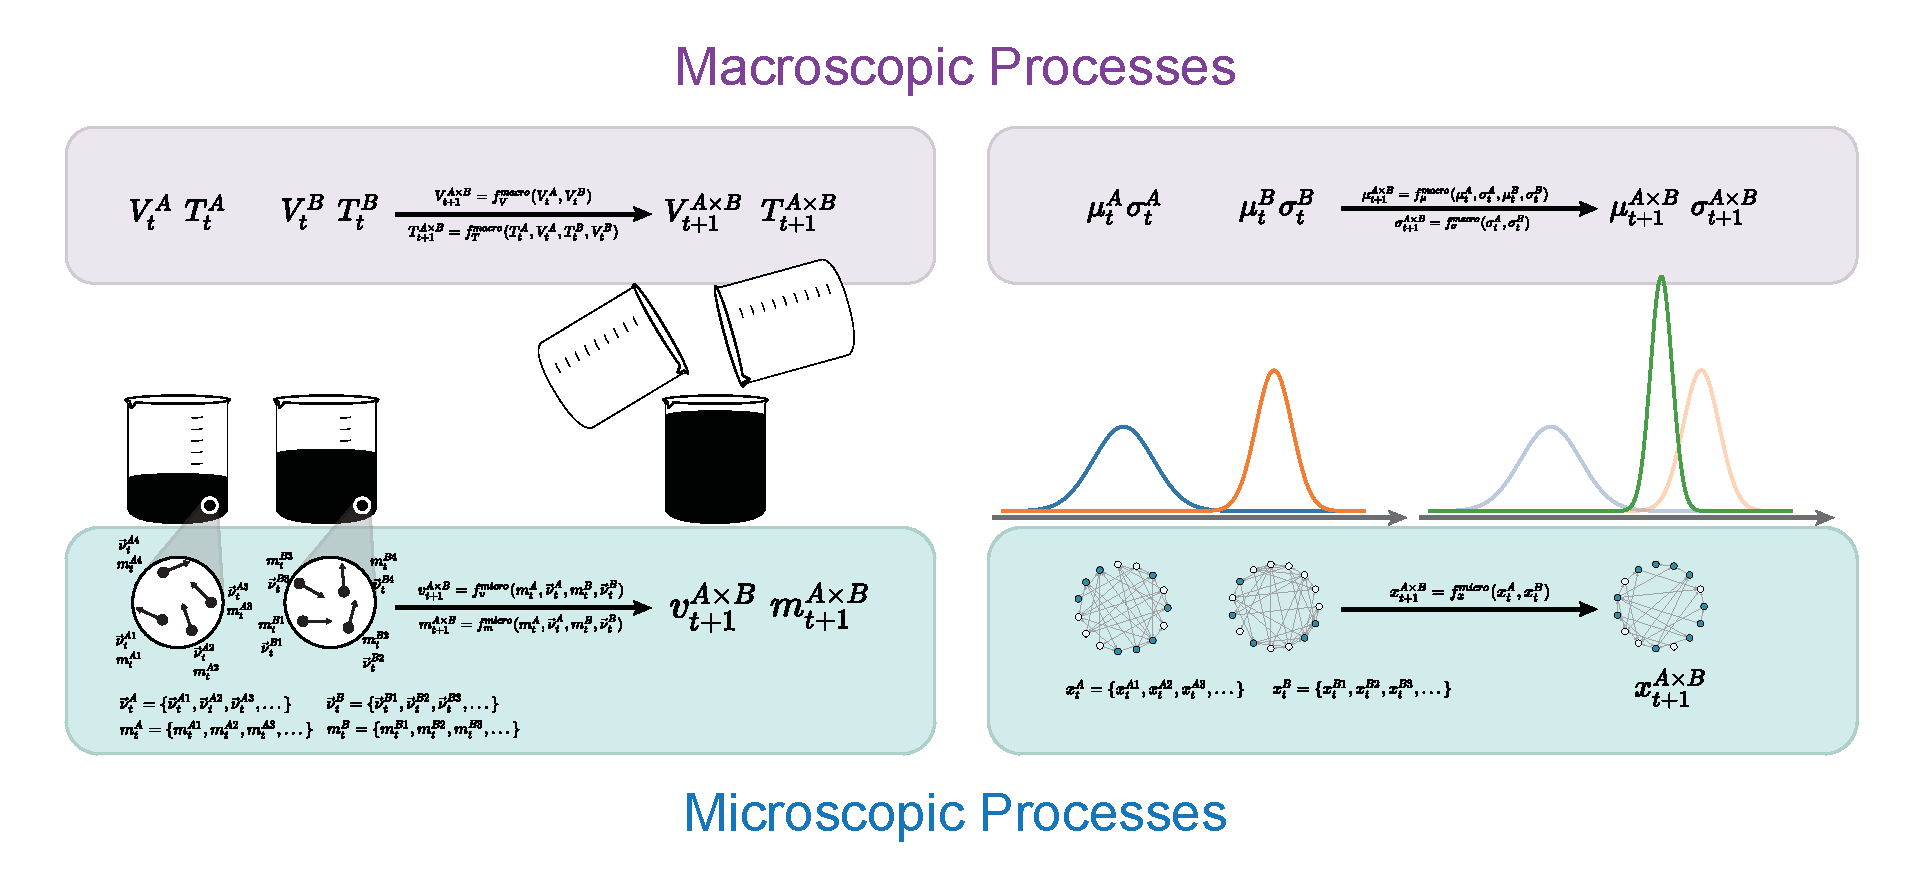
\includegraphics[width=1.3\textwidth]{WritingMaterials/Fig_Temperature_Example/ExampleOfCG.pdf}
    % 		\centering
    % 		\caption{An Example of ...}
    % 		\label{fig:TemperatureExample}
    % 	\end{figure}         
        
        
    %     The same scenario can be applied to the results from Libet's volition experimental paradigm \citep{Libet1983TimeOC, Libet1985Dec}. Experiments using similar procedures usually show that the recorded neural activities start earlier than subjects' feeling of their own intention to act in the self-determined experimental settings. We argue that free actions are initiated at the microscopic levels, for example, the random fluctuation in the neural system \citep{schurger_accumulator_2012}. However, the conscious experience of volition is information at the macroscopic level with NTIC. Due to the information closure, there is no way for the NTIC process to observe the information of the microscopic states, i.e. the initiation of actions. 
        
    
    %     \idea{Not sure if I want to address this point}  Note that, some evidence suggests single-cell-level correlation of conscious experience, the Jennifer Aniston cell for example \citep{Quiroga2005Jun, Quiroga2012Jul}. This may seem to counter our argument that single-cell level information is incapable to be conscious. However, first, the correlations are always not the direct microscopic state changes of the cells, e.g. the action potentials. Instead, the correlated variables are always coarse-grained. The neuronal firing rate, for example, is a temporal coarse-grained variable. Second, it has been well established that heterogeneous nonlinearity is critical for neural populations to encode rich and high dimensional information. \citep{Chelaru2008, Rigotti2010Oct, Shamir2004Jun}. It is common to detecting a single neuron whose activity profile well align with a subspace which represents a single object within the state space of a population code.\needhelp{Maybe need to rewording here} We believe that multi-scale data and analyses are needed to elucidate whether single neuron behaviours are sufficiently representative for any type of conscious experience. 
    
    % % ============================================================================ %
    % %                        Comparison with other theories                        %
    % % ============================================================================ %
    \section{Comparison with other Relevant Theories of Consciousness}\label{sec:Comparison with other theories}
    In this section, we compare \ac{OurTheory} with other relevant theories of consciousness.
	
	
        % ---------------------------------------------------------------------------- %
        %        Theories about multilevel views on consciousness and cognition        %
        % ---------------------------------------------------------------------------- %
        \subsection{Multilevel views on consciousness and cognition}\label{sec:MultiLevelView}
    		\ac{OurTheory} proposes that conscious processes can occur at any level of coarse-graining which forms NTIC within a system. This suggests that the scale of coarse-graining is critical for searching and identifying the information corresponding to consciousness. A few versions of multilevel views on consciousness have previously been (explicitly or implicitly) proposed. To our knowledge, Pennartz's neurorepresentational theory (also called Neurorepresentationalism,~\citep{pennartz2018consciousness,pennartz2015brain}) is the proposal closest to the multilevel view of \ac{OurTheory}. Similar to Neurorepresentationalism, the concept of levels in \ac{OurTheory} is also relevant to Marr's level of analysis~\citep{marr1982vision, pennartz2015brain, pennartz2018consciousness}. 
    		However, \ac{OurTheory} suggests that coarse-graining is necessary only when the microscopic processes are stochastic (e.g. the neural system). An NTIC process can be formed in a noise-free deterministic system without coarse-graining. According to \ac{OurTheory}, this NTIC process is sufficient to be conscious. 
    		Another fundamental difference between \ac{OurTheory} and Neurorepresentationalism is that Neurorepresentationalism takes functionalist perspective and suggests consciousness should serve high-level world-modelling and makes a best guess about the interaction between the body and the environment. 
    		%Neurorepresentationalism also suggests conscious experience is associated with integrated representation for multimodal and situational information.
    		However, \ac{OurTheory} is grounded by non-functional informational assumptions. Therefore, \ac{OurTheory} provides a more fundamental explanation for the scale problem of consciousness. 
    		
    		Another well-known proposal based on multilevel views is the Intermediate Level Theory of Consciousness \citep[ILT]{prinz2007intermediate, jackendoff1987consciousness}. ILT proposes that conscious experience is only associated with neural representations at intermediate \textbf{levels of the sensory processing hierarchy} (e.g., the 2.5D representation of visual processing) rather than lower (e.g., pixel) or higher (e.g., abstract) levels of the sensory hierarchy. 
    	
    		Here, we want to make clear that the "level" in \ac{OurTheory} refers to the \textbf{levels of coarse-graining} instead of the "level" for the cortical anatomy or sensory processing. It is important to note that the coarse-graining direction is an orthogonal dimension irrespective of the level of anatomy or the level of information processing hierarchy in the neural system (see Fig.~\ref{fig:hierarchy}). Because ILT focuses on the levels of the sensory processing hierarchy and \ac{OurTheory} focus on informational closure among the levels of coarse-graining, the two theories are fundamentally different.  
    		
    		
    		\begin{figure}[H]
    			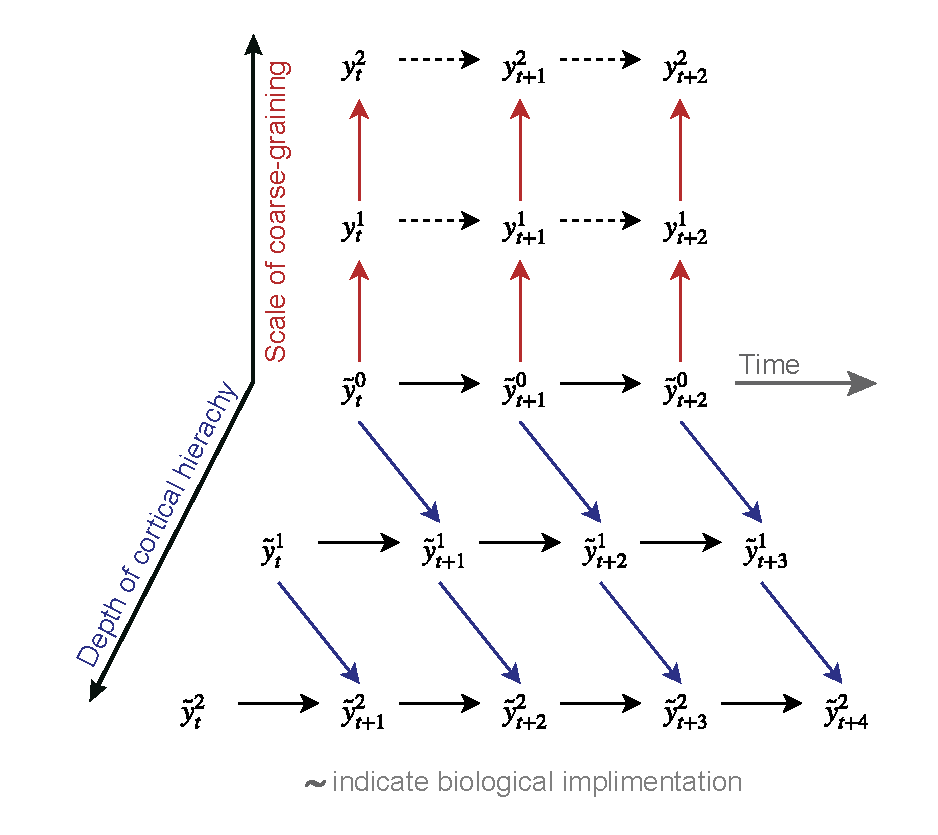
\includegraphics[width=\textwidth]{WritingMaterials/Fig_SeperationOfCGandCortHierachy/SeperationOfCGandCortHierachy.pdf}
				\caption{The distinction between the level of coarse-graining and the level of the cortical hierarchy. $X$ and $Y$ represent the microscopic and macroscopic coarse-grained  variables, respectively. $X^0$ represents the microscopic states at the upstream of the cortical hierarchy. The red empty arrows represents the directions of coarse-graining and the blue arrows represent the directions of the physical dependencies in the cortical hierarchy from the upstream to the downstream. (Some variables and dependencies are omitted for clarity.)}
				\label{fig:hierarchy}
    		\end{figure} 
    		
        
        % ---------------------------------------------------------------------------- %
        %                                      IIT                                     %
        % ---------------------------------------------------------------------------- %
		\subsection{Integrated information theory}
            Integrated information theory (IIT) states that consciousness is integrated information and system's consciousness is determined by its causal properties \citep{tononi2016integrated}. \ac{OurTheory} is in line with IIT in that informational properties are thought to underlie consciousness. In this section, we will discuss \ac{OurTheory} in the light of IIT. 
            
            \textbf{The concept of "information"}: In IIT, information refers to "integrated information":\\ \say{Information that is specified by a system that is irreducible to that specified by its parts.}~\citep{tononi2016integrated} In \ac{OurTheory}, information refers to "self-information", i.e. information about the states of conscious experience and the physical states of a process. Therefore, IIT focuses more on the relationships between consciousness and causal interactions among elements within a system, whereas \ac{OurTheory} focuses more on the informational relationships between conscious experience and being in a certain state of a process. 
		    
		    \textbf{The "Exclusion" axiom in IIT}: In IIT, the Exclusion axiom claims that of all overlapping sets of elements, only one set with maximal integrated information can be conscious. The exclusion axiom should be applied over elements, space, time, and scales \citep{oizumi2014phenomenology, hoel2016can}. Different from IIT, \ac{OurTheory} allows multiple consciousnesses coexist across different levels of coarse-graining within a system if they are informationally closed from each other. The two distinctive predictions decisively pinpoint the core concepts of the two theories. 
		    
		    \textbf{Prediction after system damaged}: \ac{OurTheory} and IIT lead to different predictions when a system suffers from a damage. For example, considering a densely connected networks whose dynamics forms an NTIC process. If we cut the network in half, IIT would predict that this results in two consciousnesses because elements in both networks still maintain high degrees of interactions. In contrast, \ac{OurTheory} would predict that this operation could completely destroy NTIC rendering both parts unconscious.
		    
		    In the current paper, we did not include the notion of integrated information within \ac{OurTheory}. However, one of the current weaknesses of \ac{OurTheory} is that it lacks the ability to individuate NTIC processes as distinct entities because a macro-process composed of two independent NTIC processes is also an NTIC. This is a severe limitation of our current theory.  The notion of integration is a possible remedy for this issue and we hope to address this more explicitly in future work using the concept of synergy. 
		    

            % ============================================================================ %
            %                                    Backup                                    %
            % ============================================================================ %

% 		    % ================================ Difference ================================ 
% 		    \begin{ants}
%     		    @@ However, \ac{OurTheory} considers that when a process is informationally closed to the universe, the process can be reckoned as a reality.

%     		    One difference is that IIT does not consider environmental information
%     		    @ IIT considered causality is the key foundation of consciousness
%     		    @ \ac{OurTheory} focus more on informational closure as the key properties to form a reality. 
% . 
    		    
    		    
%     		    @ Conscious contents in \ac{OurTheory} are 
%     		    @@  a subset of elements can contribute a specific aspect of experience only if its cause-effect repertoire within the system is irreducible by the minimum partition of the mechanism (‘small phi’ or φ)
    		    
%     		    @@ \ac{OurTheory} considered whether a part contribute conscious content whether it's within the range of informational closure
    		    
%     		    @ Exclusion 
%     		    @@ Boundary problem by exclusion
%     		    @@ In \ac{OurTheory}, boundaries of a conscious process is defined by its information boundary, i.e. informational closure.
%     		    @@ ic between level
%     		    @ conscious level
%     		    @@  Φ max
% 		    \end{ants}
		
		
% 		    % ----------------------------------------------------------------------------
%     		Integrated information theory (IIT) states that system's consciousness is determined by its causal properties. Consciousness is integrated information. As a computational theory of consciousness, the degree of discrimination and integration can be expressed in mathematical terms $\Phi$. Different from most of other scientific theory of consciousness, IIT asserts that the fundamental physical property associated with consciousness is causality.
    		
%     		% -------------------------------- Similarity -------------------------------- %
%     		IIT and our theory shares common principles in many aspects. First common principle between our theory and IIT is that instead of NCC, both theories suggest information is the fundamental entity which correlates consciousness \needref{cite David Chalmers}. Therefore, both theories are capable of extrapolation and infer the states of consciousness in other systems beyond the human neural system.
    		
%     		Second, both theories consider informational structure as the fundamental entities associated with the quality of conscious contents. IIT proposes that a "complex" which is defined as elements that generates a local maximum of integrated information as the core entity which determines the state space of subjective feeling (qualia space). In the current stage of our theory development, we have not proposed such sophisticated description of the mappting between informational structure and the qualia space. However, in line with this notion, we argue that the state space of an NTIC process determines the subjective experience possessed by the process. 
    		
    		
    		
%     		\ideaBox{Maybe synergy is the common part of the two theories }
    
%     		Even though both theories are based on informational properties of a process, predictions of the two theories can be very different. Taking the split brain cases as the example, when splitting a system into two parts, IIT suggests that each part can form a new complex. Therefore, splitting creates two new conscious entities. However, according to our theory, splitting a system may totally destroy the informational structure that created NTIC. This may lead to very small degree of NTIC in both hemispheres, thereby entirely destroying consciousness of this system. Notwithstanding, more simulation work is needed to thoroughly clarify how the two theories make same and different predictions in different contexts. Fortunately, due to the computational nature of the two theories, precise differences of predictions can be made from relatively simple toy model in the future work. 
    		
%     		% Hoel's theory\cite{hoel2016can}}
%     		Alongside with the main theoretical development of IIT, \cite{hoel2016can,hoel2013quantifying} discussed the scale-dependent causal structures using IIT as a measure of causal power at different scales. The result shows a qualitative similarity to our theory. The causal power can emerge at macroscopic levels of a system. This claim is consistent with our prediction in which processes at macroscopic levels can form more deterministic and predictive state transitions. We expect further mathematical and empirical analysis can reveal the relationship between \ac{OurTheory} and Hoel's analyses about the causal power at different scales in a system.  



        % ---------------------------------------------------------------------------- %
        %                            Predictive Processing                             %
        % ---------------------------------------------------------------------------- %
		\subsection{Predictive Processing}
    		Predictive processing (PP) is a powerful framework which integrates several ideas from neuroscience. This emerging theoretical framework posits that neural systems constantly generate predictions about incoming sensory signals and updates predictions based on prediction errors between predictions and sensory signals. According to PP, neural systems constantly perform unconscious statistical inference about hidden causes in the external environment. The perceptual contents are the "best guess" about the environment states including these hidden causes \citep{clark_2013, Hohwy2013}. PP is well integrated with Bayesian brain hypothesis and has been used to interpret conscious perception in many domains \citep{Hohwy2013, SethPP2014}.
    		
    		%% The gaps between pp and consciousness
    		PP is a powerful explanatory framework for diverse brain functions. However, to serve as a theory of consciousness, PP is still incomplete due to two explanatory gaps. First, it has been known that the neural system is equipped multiple predictive mechanisms. Apparently, not all the predictive mechanisms are involved in conscious processes (e.g. mismatch negativity, \cite{naatanen2007mismatch}). PP needs to explain the difference between conscious and unconscious predictive mechanisms. 
    		
    		Second, PP can be considered as a sophisticated computation for perceptual inference. It takes von Helmholtz's conception of perception as unconscious inference. Thus, only the most probable outcome computed by the inference processes can be conscious while other details of the computation remain unconscious. PP also needs to explain how unconscious inferences is able to give rise to conscious results. In short, while PP is often discussed in the context of consciousness, these explanatory gaps prevent PP from being a theory of consciousness. 
    		
    		% compatible things
    		\ac{OurTheory} is well compatible with PP. Crucially, \ac{OurTheory} further provides natural and fundamental explanations to fills the two explanatory gaps which PP encounters. According to the definition of NTIC, a process with high NTIC can be regarded as a powerful predictive machine which has accurate self-predictive information ($I(Y_{t+1};Y_{t})$, E.q.~\ref{eq:NTIC}) and concurrently incorporates environmental information into its dynamic ($I(Y_{t+1};Y_{t}|E_{t})$, E.q.~\ref{eq:NTIC}). This predictive nature of NTIC processes is in agreement with the core notion of PP in which the conscious contents are always the predicted (inferred) outcome of our predictive mechanisms. Second, due to the informational closure to the environment, the encoded information about its environment in an NTIC process can be seemed as "the best guess" about the external environment in the context of Bayesian inference. 
    		
    		% fill the gaps
    		So, eventually, why are some predictive information conscious and some are not? \ac{OurTheory} predicts that only the predictions generated from mechanisms involving the NTIC process are conscious. Note that predictive processes are not necessary to involve NTIC processes. A predictive process can make prediction about the future state of its environment based on the current sensory inputs. In this case, the the process is not informationally closed and could not be conscious.
    		
            According to \ac{OurTheory}, we further propose that we can only be aware of the predictions from predictive processes due to informational closure to computational details of microscopic predictive processes. The macroscopic NTIC process only acquires the coarse-grained summary statistics of the microscopic processes. In other words, we predict that the computation of the statistical inferences of PP is implemented at microscopic (cellular) levels in the neural system. 
        
    		% finally
    		Finally, we consider PP as an potential empirical implementation of NTIC processes. To maintain accurate information about the environment encoded in an NTIC process, one can open an information channel between the process and the environment for minimal information flow to correct the divergence between them. This proposal is compatible with PP which suggests that PP systems updates (corrects) the current estimations by computing prediction errors between predicted and real sensory inputs. 
    		
    		
    		
    		% ============================================================================
    		----------------------------------------------------------------------------\\
    		
    % 		Furthermore, only the mutual information between environments and NTIC processes matters. The "true" external reality may not be known. 
    		
    		
    		
    % 		self-predictive nature of a NTIC process  
    		
    		
    % 		Here, from more fundamental principles, we  argue that our theory is able to well fill the two gaps simply by considering the two conditions mentioned in section \ref{sec:Conscious versus Unconscious Processing}.
    		
    % 		First, predictive processes do not necessitate NTIC. A neural mechanisms is able to generate prediction does not guarantee it is an NTIC process. For example, an algorithm can take the current states of a target entity as the inputs and compute future states of the target. In this case, this algorithm can compute predictive information. However, the states of the internal variables are fully determined by the external input, implying that this algorithm is not informationally closed. We suggests that if a predictive process is not an NTIC process, predictions from this process will not be able to show in conscious contents (i.e., fail to meet the 1\lowercase{st} condition in section \ref{sec:Conscious versus Unconscious Processing}). In contrast, predictive information in the NTIC process is conscious and makes the process form information closure. 
    		
    % 		Second, as mentioned in section \ref{sec:Conscious versus Unconscious Processing}, if a process is not at the coarse-grained level achieving NTIC, this process will not be conscious (Fail to meet the 2\lowercase{ed} condition). We have provided an example in section \ref{sec:Conscious versus Unconscious Processing} in which computation can be implemented at microscopic levels. However, if the coarse-grained result of the computation is included in the macroscopic NTIC process, only the result rather than the process itself can be consciously aware of. Therefore, we predict that the statistical inferences under PP are implemented in microscopic levels. The NTIC process is ignorant to the detail information of their computations. 
    
    %         Altogether, our theory provides more fundamental principles and explanations about the relationship between predictive mechanisms and consciousness. Moreover, the fundamental principles allow us to make more precise predictions about which types of PP should or should not be conscious. Therefore, our theory has stronger falsifiability and predictability beyond PP on consciousness research.
        



        % ---------------------------------------------------------------------------- %
        %                           Sensorimotor contingency                           %
        % ---------------------------------------------------------------------------- %
		\subsection{Sensorimotor contingency}
    		Sensorimotor contingency (SMC) theory of consciousness proposes that different types of SMCs give rise to different characteristics of conscious experience \citep{o2001sensorimotor}. The theory radically rejects the view that conscious content is associated with internal representations of a system. Rather, the quality of conscious experience depends on agents' mastery of SMCs. SMC emphasises that the interaction between a system and its environment determines conscious experience. 
    	
    	    \ac{OurTheory} is not compatible with SMC due to the fundamental differences of assumptions of the two theories. As mentioned in Sec.~\ref{sec:Conscious versus Unconscious Processing}, a process directly maps the sensory states to the action states is insufficient to be NTIC. Therefore, learning contingencies between sensory inputs and action outputs does not imply NTIC. Hence, \ac{OurTheory} predicts that having sensorimotor contingencies is neither a necessary nor a sufficient condition for consciousness. In fact, empirically, with extensive training on a sensorimotor task with a fixed contingency, the task can be gradually performed unconsciously. This indicates that strong SMCs do not contribute conscious contents. In contrast, \ac{OurTheory} suggests that, with extensive training, the neural system establishes a neural mapping from sensory inputs to action outputs. This decrease the level of informational closure and, as a result, decrease the conscious level of this process. This outcome strongly supports \ac{OurTheory} than SMC. 
    	    
    	    Nevertheless, \ac{OurTheory} does appreciate the notion that interactions between a process and its environment is crucial to shape conscious experience. As mentioned above, to form NTIC, a process needs to encode environmental transitions into its own dynamic. Therefore, information of agent-environment interaction should also be encoded in the NTIC process, and therefore, shape conscious contents in a specific way. 
    	    
    	    Different from the classical SMC, a new version of SMC, Predictive Processing of SensoriMotor Contingencies (PPSMC), proposed by \cite{seth2014predictive, seth2015presence} PPSMC combines SMC and the predictive processing framework together. PPSMC emphasises the important role of generative models in computing counterfactual, inferring hidden causes of sensory signals, and linking fictive sensory signals to possible actions. We argue that if the generative model involving the NTIC process for the computation of counterfactual, PPSMC will be compatible to our theory and may have strong explanatory power on some special conscious experience.
    	    
    	    
    	   
        % ---------------------------------------------------------------------------- %
        %                             First-order theories                             %
        % ---------------------------------------------------------------------------- %
% 		\subsection{First-order theories}
            % The first-order theories suggest that consciousness is determined by early sensory information or neural activities\needref{First-order theories}. The first-order view maintains that conscious awareness is determined by early sensory activity alone, independently of higher-order representations.
            % First-order theories suggests that phenomenal consciousness is associated with fine-grained contents for the first-order processes. Different from the first-order theories, our theory suggests that, whether the early sensory activities show in the conscious content, it depends on information encoded in the early sensory areas is recruited in the NTIC process at the macroscopic level or not. As we mentioned in \ref{sec:Unconscious Processing}, if the sensory activities are only passively triggered by the environmental states, they are not able to form hign NTIC and remain unconscious. We predict that, if early sensory information or neural activities after coarse-graining take parts in the NTIC process, early sensory information or neural activities can contribute conscious content. 
		
		
        % ---------------------------------------------------------------------------- %
        %                 Higher Order Thought theory of consciousness                 %
        % ---------------------------------------------------------------------------- %
% 		\subsection{Higher Order Thought theory of consciousness}
% 		    \ideaBox{Okay, I don't know how to deal with HOT now. I don't understand it at all}
% 		    In contrast to first-order theories, higher-order thought theories suggest that consciousness depends on higher-order representations which represent agents as being in particular internal states \citep{lau2011empirical}. First-order processing needs to be observed or represented by a higher-order observer to become conscious. 
		    
		    
% 		    Meta-cognition is also associated with many conscious cognitive function. However, we propose a new perspective and indicate that HOT may be a misunderstanding \critical{Very bad writing. I need to rewrite this part}. 
		    
		    
% 		    This may be the result of neural coarse-graining. Because contents in informational closure look like watching fine-grained information, people may have an wrong impression about it. 
		    
		    
% 		    Coarse-grained information can be summary statistics which may be misunderstood as higher-order representation. It is true that the neural system does create  meta-representation to represent xxx\needref{Maybe come studies about confidence represenatation}. The higher-order representation may resemble coarse-grained variables. This may cause misidentify the entity which correlates conscious experience.  
		    
% 		    Moreover, the predictive information in NTIC is critical for other systems to build forward models for a wild range of tasks. Therefore, most of the high level cognition can utilise the state of informational closure. For example, mental planning needs a precise forward model to infer the environmental dynamics.

				
        % ---------------------------------------------------------------------------- %
        %                            Global workspace theory                           %
        % ---------------------------------------------------------------------------- %
        
		\subsection{Global workspace theory}
		Global workspace theory (GWT; \cite{baars1988cognitive, baars1997theatre, baars2002conscious}) or Global Neuronal Workspace theory (GNWT; \cite{dehaene1998neuronal, dehaene2001towards, dehaene2011experimental}) states that the neural system consists of several specialised modules and a central global workspace (GW) which integrates and broadcasts information gathered from those specialised modules. Only the information in the global workspace reaches conscious awareness, and information outside of it remains unconscious. These modules compete with each other to gain the access to the GW and the information from the winner triggers an all-or-none "ignition" in the GW. Information in the GW is broadcasted to other modules. Conscious contents then are associates with the information that gains access to the internal global workspace \cite{Dehaene2017}.
		
        While GWT emphasise the importance of global information sharing as a basis of consciousness, the precise meaning of information broadcasting has been somewhat unclear if one tries to describe it more formally in the language of information theory. \ac{OurTheory} offers one possible way to consider the meaning of broadcasting in GWT. Specifically, one could interpret the global workspace as the network of nodes where information is shared at the scale of NTIC where communication is performed through macro-variables that are linked via mutual predictability. That is, global workspace should be also NTIC. While this link remains speculative at this point, this interpretation encourages empirical studies into the relationship between the contents of consciousness and macrostate neural activities that are mutually predictive of each other. 
		
		
% 		=================================== Old  =================================== 
		
% 	    There are nearly no have no commonality between GWT and \ac{OurTheory}. In GWT, only information can be accessed by GW is conscious. However, it's always difficult to identify the GW because there is no clear computational definition for it. In \ac{OurTheory}, any process forming NTIC is conscious. Therefore, to determine whether a process is conscious is a decidable problem for \ac{OurTheory} but not for GWT. 
	    
% 	    GWT claims that a module is not accessed by the GW is unconscious. 
		
		
% 		Currently, we don't have strong theoretical implications to relate \ac{OurTheory} to GWT. However, based on \ac{OurTheory},  reasoning
		
% 		First, according to \ac{OurTheory}, consciousnesses occurs together with NTIC processes. Due to processes in the GW are accompanied by conscious experience, we suggest that the GW should occur at the scale where NTIC is formed. Second, notion of assess to GWS could be the state changes of the NTIC process at this coarse-grained level. Third, the all-or-none non-linear ignition may suggest the functions of coarse-graining are nonlinear. Finally, because NTIC encodes complex information about environmental states and dynamics,any state of the NTIC process can be seen as an integration of high dimensional information.
		
		
% 		P-consciousness vs A=consciousness
		
		
% 		Due to processes in the GW are accompanied by conscious experience, we can only postulate that the GW should occur at the scale where NTIC is formed. It is also likely that the 
		
% 		GWT proposes a number of core properties, e.g., stability, broadcasting, and non-linear ignition. 
		
% 		In \ac{OurTheory}, self-predictive information $I(Y_{t+1};Y_{t})$ is one of the quantity that contributes NTIC (Eq.~\ref{eq:nticObjective}). This property grantees the stability of a NTIC process. This outcome coincides with one of the GWT's claim that conscious contents often show stronger stability which may be necessary for the neural system to integrate information from a variety of modules. Although stability is claimed by both theories, the underliing reasons are different. GWT suggests that the neural mechanism to achieve stability is top-down amplifications from the GW to individual modules which gain the access to the GW. In contrast, \ac{OurTheory} suggests that stability is a natural consequence of NTIC without additional assumptions.
		
% 		We will address this comparison in our following modelling paper.
% 		Currently, we do not have concrete prediction about how an NTIC process reacts to rapid changes in the environment.
% 		More modeling work is needed 
		
		
% 		However, regarding broadcasting and non-linear ignition
		
		
		
% 		conjectures to bridge the two theories. 
		
% 		GW itself could be the NTIC process 
		
% 		similar or dissimilar 
		
		
% 		We suggests that the GW should occur at the scale where NTIC is formed. 
% 		We further hypothesise that the GW recruits the NTIC process to achieve its functional goal and, therefore, is accompany by conscious experience. 
		
% 		Self-predictive information $I(Y_{t+1};Y_{t})$ is one of the quantity that contributes  NTIC (Eq.~\ref{eq:nticObjective}). This property grantees the stability of a NTIC process. This outcome coincides with one of the GWT's claim that conscious contents often show stronger stability which may be necessary for the neural system to integrate information from a variety of modules.Although stability is claimed by both theories, the proposed reasons are different. GWT suggests that the neural mechanism to achieve stability is top-down amplifications from the GW to individual modules which gain the access to the GW. In contrast, \ac{OurTheory} suggests that stability is a natural consequence of NTIC withour additional assumptions.
		
% 		The notion of assess to GWS could be the access at the coarse grained level. 
		
% 		We suggest that when a coarse-grained variable becomes a part of the NTIC process. This makes information about the states of the variable occur in the conscious contents. 
		
		
		% ================================= Super old ================================ %
		
		    
% 		\needhelp{I think I need some help here. I am not sure what should I write here. Or  what position I should take. To some extent, GWT is a very qualitative theory. It kind of just summarises everything. Without any modelling work on NTIC, it's difficult to say whether we will replicate those profiles of consciousness mentioned in GWT.}
% 		\ideaBox{Need ending and better difference }
% 		Global workspace theory (GWT; \cite{baars1988cognitive, baars1997theatre, baars2002conscious}) or Global Neuronal Workspace theory (GNWT; \cite{dehaene1998neuronal, dehaene2001towards, dehaene2011experimental}) states that the neural system consists of several specialised modules and a central global workspace (GW) which integrates and broadcasts information amount these modules. Only the information accessed by the global workspace can be consciously aware of. These modules competes with each other to gain the access to the GW and the information from the winner can trigger an all-or-none "ignition" in the GW. Information in the GW is able to be broadcasted to other modules. Conscious contents then associates information which gains access to the internal global workspace \cite{Dehaene2017}.
		
% 		In many aspects, our theory can well accommodate GWT. NTIC processes shares several properties with the GW. Here we discuss three core properties, stability, broadcasting, and non-linear ignition, emphasised by the GWT. 

% 		% === Stability ===
% 		Stability: GWT indicates that the conscious contents often show stronger stability which may be necessary for the neural system to integrate information from a variety of modules. Suggested by GWT, this is caused by top-down amplification from the GW to individual modules which gain the access to the GW \needref{}. In contrast, without assuming any additional mechanism, our theory argues that stability is a natural quality of NTIC due to its strong self-predictive characteristic. Our theory can even further quantify the stability of conscious contents by computing the mutual information between the current and the future states of a conscious process. 
		
% 		% === Broadcasting ===
% 		\idea{A bit not sure about this part}Broadcasting: Because individual modules use different coding schemes, the neural system requires a mechanism for passing information between modules. GWT suggests that the GW is responsible for connecting the information source, translating the code, and finally making the information globally accessible. We argue that, because the NTIC process encodes high dimensional information about the environmental dynamics, it can be considered as an integrated informational entity \todo{Need rewording}. These with the coarse-graining variables involved in the NTIC process together. Other modules outside the NTIC process can decode and extract needed information for the current goal of the task. 
        
        
%         % === Non-linear ignition ===
%         Non-linear ignition: Non-linear ignition: Because mapping microscopic to macroscopic states is many-to-one, it commonly shows a nonlinear relationship between microstates and macrostates \needhelp{Is this statement correct?}. Therefore, a continuous state transition at microscopic levels may lead to a discrete and non-linear state transition at macroscopic levels. Based on our theory, when new information enters conscious contents, the NTIC process must undergo a corresponding state transition. This transition can trigger a significant change of the brain states and resembles non-linear ignition of brain activities
        
        
%         \idea{Long distance connectivity?}
%         \rewrite{(1) sudden, all-or-none ignition of prefronto-parietal networks; (2) concomitant all-or-none amplification of sensory activation; (3) a late global P3b wave in event-related potentials; (4) late amplification of broad-band power in the gamma range; (5) enhanced longdistance phase synchronization, particularly in the beta range; and (6) enhanced causal relations between distant areas, including a significant top-down component. }
%         Future modeling work is needed

% 		% -------------------------------- Difference -------------------------------- %
% 		\todo{Finish this part}
% 		However, there are still fundamental differences between the two theories. 
% 		In GWT, modules rival with each other to gain access to the GW. Our theory suggests that the one enters conscious contents is the one which can create the higher NTIC with other coarse-grained information. This difference leads very different predictions and implications. For GWT, to find the biological implementation of the rivalry mechanism (attention, for example) is critical. However, we do not assume any rivalry mechanism. Instead, we argue that, if  information carried by the coarse-grained variables can increase the predictability of the process and form high NTIC,  it naturally form a informationally closed boundary and 
		
% 		Up to now, GWT does not indicate in what conditions a process can be considered as a GW. This results in an intractable situation of finding the GW, especially when empirical data show distributed information encoded in many brain areas\citep{siegel2015cortical}. 
		
% 		Another difference between our theory and GWT is that our theory does not suggest a neuronal core anatomical area for consciousness. \todo{Link to Section 4}. Coarse-grained information in NTIC is more crucial for consciousness rather than neural substrates supporting the global workspace.
		
% 		In sum, our theory is compatible with previous physiological evidence supporting GWT.  





% ============================================================================ %
%                                  Limitation                                  %
% ============================================================================ %
    \section{Limitation and Future work}\label{sec:Limitation and Future work}  
        In this article, we propose the first version of \ac{OurTheory} and introduce the central concepts, assumptions, and propositions. However, as a brand new theory of consciousness, \ac{OurTheory} is still far from completion. In the following, we discuss the current limitations and challenges of \ac{OurTheory} and point out the potential future research directions.
    
        % =============================== Theoretical  ===============================
        
        % Can't solve the hard problem
        It's important to clarify that \ac{OurTheory} does not intend to completely solve the hard problems of consciousness \citep{chalmers1995facing}. Knowing the state of a conscious process does not allow us to answer "What is it like to be in this state of this process" \citep{nagel1974like}. Instead, \ac{OurTheory} focuses more on bridging consciousness and the physical world using information as a common language in between. %Therefore, \ac{OurTheory} cannot solve the inverted spectrum argument \citep{Shoemaker1982-SHOTIS, Block1990-BLOIE, Locke1979-LOCTCE-2} unless we can gain one more bit of information to distinguish whether the two processes are same or different. 
        
        %This means \ac{OurTheory} cannot solve the inverted spectrum argument \citep{Shoemaker1982-SHOTIS, Block1990-BLOIE, Locke1979-LOCTCE-2}.
        
        % Identity problem
        The current version of \ac{OurTheory} cannot entirely solve the problem of individuality in some extreme circumstances. In common cases, one can identify individual consciousnesses by computing the levels of NTIC of a process. This approach can also be applied to finding the boundaries of individual consciousnesses (for details of the boundary detection procedure, see \cite{krakauer2014information}). However, in some spacial circumstances, individuality of consciousness has more than one outcome. For instance,
            \needhelp{@Martin, if you think it's better to have a proof for this and if you don't mind, you can help me to write the proof here or create an appendix section and put it there. If you have no time, I can also do this.}
        we can define a new process $Y$ and also its environment $E$ by recruiting two independent NTIC processes $Y^1~\&~Y^2$ and their environments $E^1~\&~E^2$, respectively. So that $Y = \{Y^1,Y^2\}$ and $E=\{E^1,E^2\}$. In such case, the new process $Y$ will also be NTIC to $E$. Therefore, the current version of \ac{OurTheory} cannot determine whether there are two smaller consciousnesses or one bigger consciousness (or 3 coexisting consciousnesses ). The problem of individuality is a significant theoretical weakness of the current version of \ac{OurTheory}. An intuitive solution is to recruit an "integration" quantity in our propositions. In our next theoretical article, we will discuss informational synergy and redundancy in the context of NTIC and consciousness. 
        
        % About the environment
        The current version of \ac{OurTheory} assume that consciousness is only contributed by  non-trivial rather than trivial information encoded in a process. In other words, how much information about environmental states and dynamics encoded in a process is a key quantity for consciousness. However, we do not exclude the possibility that environmental information may be just a proxy of other informational quantities. So far, we can only claim NTIC is sufficient for consciousness. We are not able to draw further speculations. More theoretical work is needed. This issue will also be discuss in our next theoretical paper. 
        
        
        
        
        
        % ================================= Empirical ================================ 
        % finding the coarse-graining function 
        Empirically, a major challenge to \ac{OurTheory} is to find proper coarse-graining functions which map microscopic processes to macroscopic NTIC processes. This will become an imperative issue of find neurological supporting evidence for \ac{OurTheory}. To find proper coarse-graining functions among infinite candidates \citep{price2007causation} seem to be very challenging. Nevertheless, there are still theoretical and technical progresses recently that may contribute to  solving this issue. For example, the concept of \textit{causal emergence} proposed by Hoel \citep{Hoel19790, Hoel2018} has been further developed recently. Causal emergence is highly relevant to informational closure at coarse-grained levels. In their new study by \cite{klein2019uncertainty}, they started to compare how different coarse-graining functions influence causal emergence at macroscopic levels. \cite{PFANTE.2014, PFANTE.2014b} provides thorough mathematical analyses on level identification including informational closure. In neuroscience, the understanding of neural population codes also achieves a tremendous progress due to the advancement of recording technique and data science \citep{Kohn2016, panzeri2015neural}. \cite{Gamez2016} has also systematically describe relevant issues in terms of finding data correlates of consciousness amount different levels of abstraction. We believe that interdisciplinary research is required to narrow down the scope of searching the coarse-graining functions and conscious processes at the coarse-grained level in the neural system and beyond. 
        
        Finally another empirical challenge to \ac{OurTheory} is the lack of empirical supporting evidence. This is understandable because the concept of NTIC is relatively new in the history of information science, not to mention in neuroscience. Very few experiments and data collections are designed for examining NTIC properties in the neural system. To our knowledge, only two studies \citep{Palmer2015, sederberg2018learning} coincidentally examine similar properties in salamander retina. They found that the a large group of neural populations of retinal ganglion cells encoded predictive information about external stimuli also had high self-predictive information about their own future states. The results, in line with the characteristic of NTIC. We expect that there will be more empirical studies examining the NTIC property in the neural system. 

% ============================================================================ %
%                                  Conclusion                                  %
% ============================================================================ %
    \section{Conclusion}
    % short re-introduction 
    In this paper, we introduced \textbf{\acf{OurTheory}}, a new informational theory of consciousness. Based on four assumptions, \ac{OurTheory} proposes that a process which forms \textbf{non-trivial informational closure (NTIC)} is sufficient to be conscious and through coarse-graining the neural system forms a NTIC process, i.e., a conscious process, at a certain macroscopic level. \ac{OurTheory} considers that information is a common language to bridge the gap between conscious experience and the physical reality. Using information theory, \ac{OurTheory} proposes computational definitions for both conscious level and conscious content. This makes \ac{OurTheory} be able to generalise to any system beyond the human brains. 
    
    % For neuroscience
    \ac{OurTheory} provides explanation for various findings from research of conscious and unconscious processing. The implications of \ac{OurTheory} point out that the levels of coarse-graining play a critical role in searching for neural substrates of consciousness. Improper measurements, e.g., too fine or too coarse in terms of the scale of measurements, of neurophysiological signals may lead to misleading results and interpretations. 
    
    
    % For scientific theory of consciousness
    \ac{OurTheory} reconciles several theories of consciousness. \ac{OurTheory} indicates that they conditionally coincide with \ac{OurTheory}'s implications and predictions but, however, not the fundamental and sufficient conditions for consciousness. For example, theories includes the theories emphasising recurrent circuits \citep{lamme2006towards, edelman1992bright}, the theories highlighting the internal simulation,  predictive mechanism, and generative models ~\citep{revonsuo2006inner, clark_2013,Hohwy2013,SethPP2014, kanai_chang_yu_de_abril_biehl_guttenberg_2019, seth2014predictive, seth2015presence}, and theories related to multilevel view of consciousness~\citep{pennartz2018consciousness,pennartz2015brain,prinz2007intermediate, jackendoff1987consciousness}. Notably, \ac{OurTheory} is proposed based on non-functional assumptions and propositions. Notwithstanding, its implications for the functional aspects of a system well fit the proposals from functionalist theories mentioned above. 
	
	
	% For philosophy of mind
	Regarding philosophy of mind, \ac{OurTheory} connects several distinct arguments together. \ac{OurTheory} can be seen as an identity theory because it assumes a fundamental relation between consciousness and information. Second, the implications of \ac{OurTheory} tightly link consciousness to several cognitive functions in the context of evolution. This explains why people might intuitively have a functionalist point of view of consciousness. \ac{OurTheory} emphasises that informational closure between levels of coarse-graining is critical to form NTIC processes in some stochastic systems. In this case, especially for the neural system, forming conscious processes at the macroscopic levels coincide with the perspective of emergentism. Finally, forming NTIC (conscious) processes through many-to-one maps, i.e., coarse-graining, implies multiple realizability of consciousness. As a result, \ac{OurTheory} provides a integrated view for these arguments and is further capable of indicating how and why they are conditionally true.

	% Final 
	So far, the current version of \ac{OurTheory} is still far from completion. Further theoretical and empirical research is indispensably required for \ac{OurTheory} to improve and solve several issues in the current version. Nevertheless, \ac{OurTheory} offers explanation and prediction for consciousness science. We hope that \ac{OurTheory} provides a new way of thinking and understanding neural substrates of consciousness.  
	
%     ================================ Old version ===============================
% 	In this paper, We introduced a new computational theory of consciousness based on two assertions. First, consciousness occurs when a process forms an NTIC. Second, in the neural system, construction of an NTIC process requires coarse graining. From these assumptions, it follows that consciousness only appears at a certain macroscopic level which forms a high degree of NTIC. 	Our  theory offers an explanation for a large number of empirical findings in consciousness research and reconciles with several other theories of consciousness. 
	
% 	Our theory asserts that consciousness is an informational phenomenon. We further emphasise that the scale-dependent nature of information processing is critical to conscious experience. We believe that many discrepancies in previous studies of neural correlates of consciousness resulted from measurements at inappropriate scales. Except where and when, future studies should also focus on "what scale" of the neural system the data are acquired at.
	
% 	The computational nature of the theory makes it feasible to extrapolate and apply to other non-human systems. Note that, even though our theory does not start from a functionalist point of view, it comes out with explanatory power on the functional aspect of consciousness and points out the evolutionary drive of having conscious processing. 
	

	
% 	Finally, we quote the famous epistemological questions: "If a tree falls in a forest and no one is around to hear it, does it make a sound?". Now, we can ask a new version of this question: "If an action potential rises outside an informationally closed process, does it make any conscious percept to this process?" We answer: "if the process is conscious, the event occurring outside the realm of the informational closure should never become part of the conscious contents."
    
    
	% ============================================================================ %
	%                                      End                                     %
	% ============================================================================ %

	\section*{Funding}
        \needhelp{@Ryota, could you help me with this part?}
	\section*{Acknowledgements}

	\section*{Supplemental Data}

	\bibliographystyle{authordate1}
	\bibliography{ref}


\end{document}
